\documentclass[conference]{IEEEtran}
\usepackage[T1]{fontenc}
\usepackage{graphicx}
\usepackage{booktabs}
\usepackage{tabularx}
\usepackage{xcolor}
\usepackage{tikz}
\usetikzlibrary{positioning,fit,arrows.meta,backgrounds}
\usepackage[hidelinks]{hyperref}
\usepackage{url}

\graphicspath{{figures/}}

% \screenshot{file}{caption}{label}: includes figures/<file> if it exists,
% otherwise a framed placeholder, so the report always builds.
\newcommand{\screenshot}[3]{%
  \begin{figure}[!t]
    \centering
    \IfFileExists{figures/#1}{%
      \includegraphics[width=\columnwidth]{#1}%
    }{%
      \fbox{\parbox[c][3.2cm][c]{0.92\columnwidth}{\centering\small
        \textcolor{red}{TODO: screenshot}\\\texttt{figures/#1}}}%
    }
    \caption{#2}
    \label{#3}
  \end{figure}}

\newcommand{\repo}{https://github.com/SisyphusRex/cloud-computing-semester-project}

\begin{document}

\title{Lecture Indexer: Prototype Review\\[0.4ex]
{\large CS 6030 Cloud Computing --- Semester Project, Milestone 2}}

\author{
\IEEEauthorblockN{Theodore Podewil}
\IEEEauthorblockA{Dept. of Computer Science\\Western Michigan University\\Kalamazoo, MI, USA}
\and
\IEEEauthorblockN{Joshua Jubenville}
\IEEEauthorblockA{Dept. of Computer Science\\Western Michigan University\\Kalamazoo, MI, USA}
\and
\IEEEauthorblockN{Andrew Wojciechowski}
\IEEEauthorblockA{Dept. of Computer Science\\Western Michigan University\\Kalamazoo, MI, USA}
}

\maketitle

\begin{abstract}
Milestone 2 asks for an initial deployment, a CI/CD pipeline, and basic
functionality. Lecture Indexer (LI) has all three. The system runs in
production on Google Cloud, with Microsoft Azure as the second provider,
and all of its infrastructure is defined in Terraform. A GitHub Actions
pipeline tests every change and releases to production after one team
approval. The core workflow from our proposal works end to end: a professor
registers a YouTube lecture, and a student searches it and jumps to the
moment a term is spoken.
\end{abstract}

\begin{IEEEkeywords}
cloud-native, multi-cloud, Kubernetes, CI/CD, Terraform, GitHub Actions.
\end{IEEEkeywords}

\section{Introduction}
LI makes recorded lectures searchable. It retrieves the timed captions of a
course's YouTube videos, indexes them, and returns links that open each
video at the moment a search term is spoken~\cite{m1}. This report covers
the prototype we built for Milestone~2. Table~\ref{tab:summary} summarizes
how we met each deliverable, and the following sections describe each one.
Source code, workflow runs, and releases are public at \url{\repo}.

\begin{table}[!t]
\caption{Milestone 2 deliverables}
\label{tab:summary}
\centering\small
\begin{tabularx}{\columnwidth}{@{}lX@{}}
\toprule
Deliverable & How we met it \\
\midrule
Initial deployment & Production environment on Google Cloud and Azure, provisioned with Terraform and running live \\
CI/CD pipeline & Automated tests on every change; one-approval releases with automatic rollback; three releases shipped \\
Basic functionality & Sign-in, lecture registration, search, and deep links, tested end to end in production \\
\bottomrule
\end{tabularx}
\end{table}

\section{Architecture}
Fig.~\ref{fig:arch} shows the system as deployed. A React web app, hosted
on Cloud Run, calls two containerized Flask services on Google Kubernetes
Engine (GKE): an Ingest API that registers lectures and a Search API that
answers queries. Each service scales independently. They share a Cloud SQL
for PostgreSQL database, whose built-in full-text search provides the index.
Users sign in with their Google accounts. Secrets are kept in Secret
Manager, and the services reach Google Cloud without stored keys.

\begin{figure*}[!t]
\centering
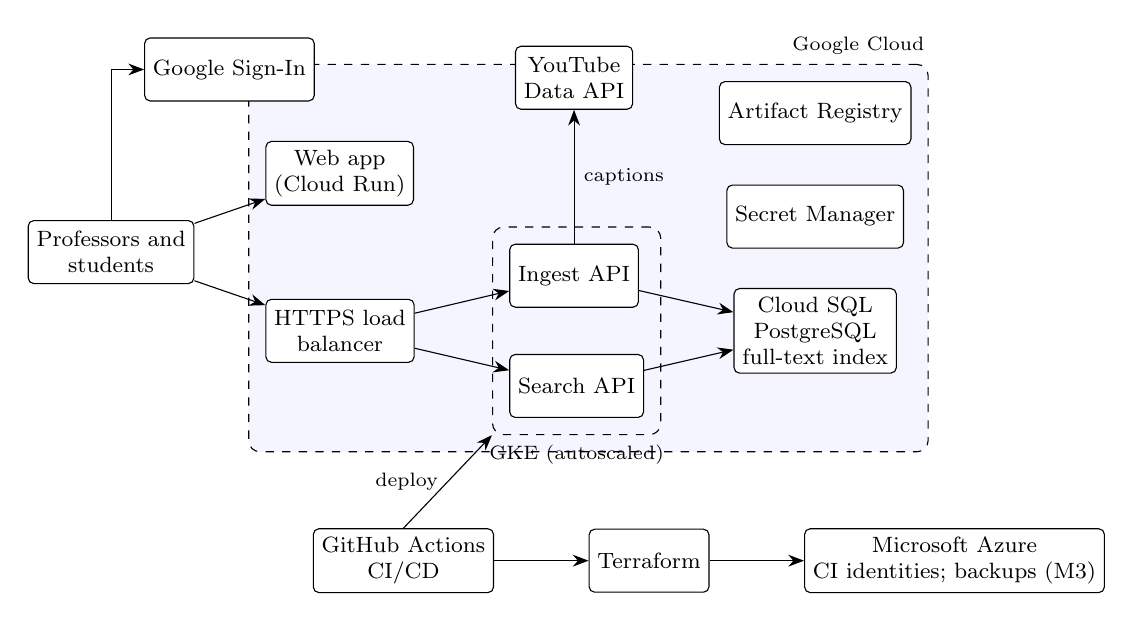
\begin{tikzpicture}[
  font=\footnotesize,
  box/.style={draw, rounded corners=2pt, align=center, minimum height=8mm, inner sep=3pt, fill=white},
  cloud/.style={draw, dashed, rounded corners=4pt, inner sep=6pt},
  arr/.style={-{Stealth[length=2mm]}},
  node distance=6mm and 9mm]
  \node[box] (users) {Professors and\\students};
  \node[box, right=of users, yshift=10mm] (run) {Web app\\(Cloud Run)};
  \node[box, right=of users, yshift=-10mm] (lb) {HTTPS load\\balancer};
  \node[box, right=12mm of lb, yshift=7mm] (ingest) {Ingest API};
  \node[box, right=12mm of lb, yshift=-7mm] (search) {Search API};
  \node[box, right=12mm of ingest, yshift=-7mm] (sql) {Cloud SQL\\PostgreSQL\\full-text index};
  \node[box, above=5mm of sql] (sm) {Secret Manager};
  \node[box, above=5mm of sm] (ar) {Artifact Registry};
  \node[cloud, fit=(ingest)(search), label={[font=\scriptsize]below:GKE (autoscaled)}] (gke) {};
  \node[box, above=5mm of run, xshift=-14mm] (gsi) {Google Sign-In};
  \node[box, above=5mm of ingest, yshift=12mm] (yt) {YouTube\\Data API};
  \node[box, below=14mm of search, xshift=-22mm] (gh) {GitHub Actions\\CI/CD};
  \node[box, right=12mm of gh] (tf) {Terraform};
  \node[box, right=12mm of tf] (az) {Microsoft Azure\\CI identities; backups (M3)};
  \begin{scope}[on background layer]
    \node[cloud, fill=blue!4, fit=(run)(lb)(gke)(sql)(sm)(ar), label={[font=\scriptsize]above right:Google Cloud}] {};
  \end{scope}
  \draw[arr] (users) -- (run);
  \draw[arr] (users) -- (lb);
  \draw[arr] (users) |- (gsi);
  \draw[arr] (lb) -- (ingest);
  \draw[arr] (lb) -- (search);
  \draw[arr] (ingest) -- (sql);
  \draw[arr] (search) -- (sql);
  \draw[arr] (ingest) -- node[right, font=\scriptsize]{captions} (yt);
  \draw[arr] (gh) -- (tf);
  \draw[arr] (tf) -- (az);
  \draw[arr] (gh.north) -- node[left, font=\scriptsize]{deploy} (gke.south west);
\end{tikzpicture}
\caption{The deployed architecture. The application runs on Google Cloud.
Azure holds the CI identities and, from Milestone~3, the off-site database
backups. GitHub Actions and Terraform deploy to and provision both clouds.}
\label{fig:arch}
\end{figure*}

\textbf{Changes from the proposal.} The proposal placed the web app on
Azure Static Web Apps. Our student Azure subscription cannot create that
service in any region it allows, so the web app moved to Cloud
Run~\cite{adr1}. Azure remains our second provider: it holds the identities
the pipeline uses, and it will store the nightly backups. We also made
sign-in invite-only, with roles managed by admins inside the app~\cite{adr2}.

\section{Deliverable 1: Initial Deployment}
\label{sec:deploy}
All infrastructure is written in Terraform and can be rebuilt from the
repository~\cite{runbook}. Terraform creates the network, the GKE cluster,
the database, the container registry, the secrets, and the Cloud Run
service on Google Cloud, plus the resource groups and identities on Azure.
The Kubernetes configuration is versioned as well, including the
autoscaling rules, network policies, and HTTPS ingress.

The environment has run in production since October 18, 2026.
Figs.~\ref{fig:gke}--\ref{fig:azure} show the services running on GKE and
Cloud Run and the Azure identities. Because a student budget is limited,
one command pauses the paid resources between test sessions without losing
any data. This cuts the idle cost to a few dollars a month.

\screenshot{fig-gke.png}{The Ingest and Search services running on GKE,
each healthy and autoscaled.}{fig:gke}

\screenshot{fig-cloudrun.png}{The web app on Cloud Run: each release
creates a new revision, and traffic moves to it only after a health
check passes.}{fig:cloudrun}

\screenshot{fig-azure.png}{Azure, the second cloud provider: the identities
the release pipeline signs in as.}{fig:azure}

\section{Deliverable 2: CI/CD Pipeline}
\label{sec:cicd}
The pipeline runs on GitHub Actions in two stages~\cite{release}:
\begin{itemize}
\item \textbf{Continuous integration.} Every push and pull request runs
linting and the automated tests, builds the container images, and checks
the Terraform and Kubernetes configuration (Fig.~\ref{fig:ci}).
\item \textbf{Continuous delivery.} Every merge to \texttt{main} starts a
release (Fig.~\ref{fig:release}). The pipeline first shows the changes and
the infrastructure plan. A team member approves once, and the pipeline then
updates the infrastructure, backs up the database if needed, builds and
deploys the services and the web app, and tags the release. If any step
fails, it rolls back automatically, and an earlier release can be restored
at any time.
\end{itemize}
The pipeline stores no cloud passwords or keys. It signs in to Google Cloud
and Azure with short-lived OIDC tokens.

The pipeline has shipped three releases so far. The first one needed a few
attempts, as we found and fixed configuration problems. Each failed attempt
stopped safely and left the running system untouched, which is what the
pipeline was designed to do.

\screenshot{fig-ci-run.png}{A passing CI run: tests, images, and
configuration checks.}{fig:ci}

\screenshot{fig-release-run.png}{A release run, from the change review and
infrastructure plan through deployment and tagging.}{fig:release}

\section{Deliverable 3: Basic Functionality}
\label{sec:func}
The prototype supports the full workflow from our proposal:
\begin{enumerate}
\item Users sign in with Google. Only invited users get in
(Fig.~\ref{fig:signin}).
\item A professor creates a course and registers a lecture from their own
YouTube channel (Fig.~\ref{fig:manage}). LI downloads the captions, cleans
them, and indexes them.
\item A student searches the course and gets ranked, highlighted excerpts.
Each excerpt plays the video at the matching moment (Fig.~\ref{fig:search}).
\item Admins invite users and assign roles (Fig.~\ref{fig:admin}).
\end{enumerate}

\screenshot{fig-signin.png}{Google sign-in.}{fig:signin}
\screenshot{fig-manage.png}{The Manage page, where professors create courses and register lectures.}{fig:manage}
\screenshot{fig-search.png}{Search results with highlighted excerpts and the embedded player at the matching moment.}{fig:search}
\screenshot{fig-admin.png}{The Admin page for invitations and roles (email addresses redacted).}{fig:admin}

\textbf{Testing.} We tested the workflow with real Google and YouTube
accounts, first locally and then in production~\cite{yttest}. The tests
covered registering a video, searching it as a student, re-registering and
deleting lectures, and confirming that a professor cannot register someone
else's video. Over 120 automated tests run on every change.

\section{Next Steps}
Milestone~3 adds the remaining pieces from the proposal: nightly encrypted
database backups to Azure, a monitoring dashboard with alerts, and a
written security review.

\begin{thebibliography}{9}
\bibitem{m1} T. Podewil, J. Jubenville, and A. Wojciechowski, ``Lecture Indexer: A multi-cloud service for timestamped keyword search of recorded lectures,'' CS 6030 Milestone 1 proposal, Western Michigan Univ., 2026.
\bibitem{adr1} ``ADR 0001: Host the frontend on Cloud Run instead of Azure Static Web Apps,'' \url{\repo/blob/main/docs/architecture_decision_records/0001-frontend-on-cloud-run.md}
\bibitem{adr2} ``ADR 0002: Invite-only sign-in, with roles set by admins in the database,'' \url{\repo/blob/main/docs/architecture_decision_records/0002-invite-only-users-and-admin-roles.md}
\bibitem{runbook} ``Bootstrap runbook'' and ``First deployment,'' \url{\repo/tree/main/docs}
\bibitem{release} ``Release process,'' \url{\repo/blob/main/docs/release-process.md}; releases: \url{\repo/releases}
\bibitem{yttest} ``Real Google/YouTube test: progress log,'' \url{\repo/blob/main/docs/milestones/m2_prototype_review/real-youtube-test.md}
\end{thebibliography}

\end{document}
